\section{Venstreorientert (leftist) heap}
En venstreorientert heap er en en heap med et annet strukturkrav enn vanlig heap. Motivasjonen bak venstreorienterte heaper er at å flette (merge) to heaper av samme størrelse tar $ O(n) $ tid, vi ønsker å forbedre det. Før vi kan definere en venstreorientert heap må vi definere \say{null path length} (herfra: npl).
\newpage
\begin{definition}
	Npl til en node $ n $ er lengden av den korteste veien fra $ n $ til en etterkommer uten to barn ($ 0 $ hvis $ n $ har $ <2 $ barn). 
\end{definition}

\begin{figure}[h!]
	\centering
	\caption{Et tre med $ \text{npl}(n) $ skrevet inn}
	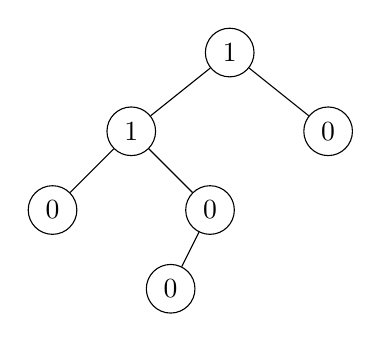
\begin{tikzpicture}[level distance=1cm,
	level 1/.style={sibling distance=2.5cm},
	level 2/.style={sibling distance=2cm},
	level 3/.style={sibling distance=1cm},
	every node/.style = {shape=circle, draw, align=center}]
	
	\node{1}
	child {
		node {1}
		child {
			node {0}
		}
		child {
			node {0}		
			child {
				node {0}
			}
			child[missing]
		}
	}
	child {
		node {0}
	};
	\end{tikzpicture}
\end{figure}

\noindent Vi er nå klare til definisjonen av venstreorientert heap:

\begin{definition} \label{def:leftheap} En venstreorientert heap er et binært tre der følgende krav er oppfylt:
\begin{enumerate}
\item For hver node $ n $ i treet er $ \text{npl}(l) \geq \text{npl}(r) $, der $ l $ er venstre og $ r $ er høyre barn til $ n $.
\item En node har alltid (sorterings)verdi mindre enn, eller lik sine barn. 
\end{enumerate}
\end{definition}



\noindent \textbf{Merk:} En venstreorientert heap forsøker å være ute av balanse (for å gjøre fletting enklere).




\subsection{Fletting, innsetting og sletting}
Hovedoperasjonen på venstreorienterte heaper er \textbf{fletting} (engelsk: merging). Fletting er forklart i teorem \ref{def:heapmerge}

For å \textbf{sette inn} en node i en venstreorientert heap kan vi flette en heap bestående av den ene noden vi vil sette inn, med hele heapen vi vil sette noden inn i.

For å \textbf{fjerne} minste node kan vi ta vekk rota (som vi vet er minst fra def. pt. 2), og flette venstre og høyre subheap.

\newpage
\begin{theorem}\label{def:heapmerge}
	La $ H_1 $ og $ H_2 $ være to venstreorienterte heaper. Vi definerer fletting reukursivt:
	\begin{itemize}
		\item Sammenlign rota i $ H_1 $ og $ H_2 $. Antar videre at $ H_1 $ er minst.
		\item La høyre subheap til $ H_1 $ være heapen som framkommer av å flette høyre subheap av $ H_1 $ med $ H_2 $. Fortsett slik til problemet er trivielt.
		\item Underveis i oppnøstinga etter rekursjonen kan høyre og venstre supheap swapes for å opprettholde strukturkrav 1 i def \ref{def:leftheap}
	\end{itemize}
\end{theorem}

\begin{example}
	Flett følgende to venstreorienterte heaper:
	\begin{figure}[H]
		\centering
		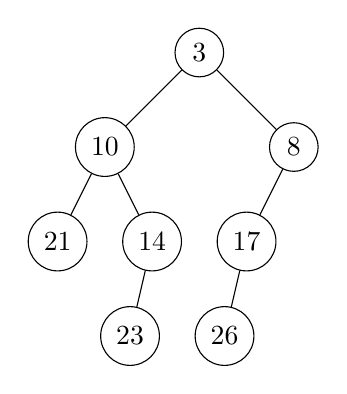
\begin{tikzpicture}[level distance=1.5cm,
		level 1/.style={sibling distance=3.0cm},
		level 2/.style={sibling distance=1.5cm},
		level 3/.style={sibling distance=0.7cm},
		every node/.style = {shape=circle, draw, align=center}, scale=0.8]
		
		\node{3}
		child {node {10}
			child {node {21}}
			child {node {14}
				child {node {23}}
				child [missing]{}
			}
		}
		child {node {8}
			child {node {17}
				child {node {26}}
				child [missing] {}
			}
			child [missing]{}
		};
		\end{tikzpicture}\quad
		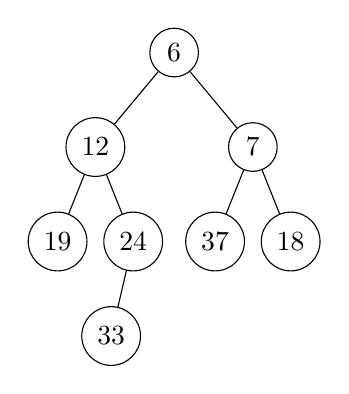
\begin{tikzpicture}[level distance=1.5cm,
		level 1/.style={sibling distance=2.5cm},
		level 2/.style={sibling distance=1.2cm},
		level 3/.style={sibling distance=0.7cm},
		every node/.style = {shape=circle, draw, align=center}, scale=0.8]
		
		\node{6}
		child {node {12}
			child {node {19}}
			child {node {24}
				child {node {33}}
				child [missing]{}
			}
		}
		child {node {7}
			child {node {37}}
			child {node {18}}
		};
		\end{tikzpicture}
	\end{figure}
	\noindent Vi kaller heapen til venstre for $ H_1 $ og heapen til høyre for $ H_2 $. Vi begynner med å sammenligne røttene (steg 0): $ 3 < 6 $, så fletter høyre subheap av $ H_1 $ med $ H_2 $, altså:
		\begin{figure}[H]
			\centering
			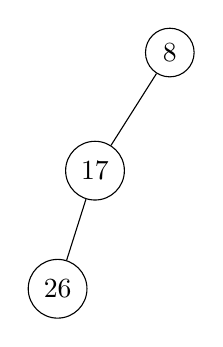
\begin{tikzpicture}[level distance=1.5cm,
			%level 1/.style={sibling distance=3.8cm},
			level 1/.style={sibling distance=1.9cm},
			level 2/.style={sibling distance=0.95cm},
			every node/.style = {shape=circle, draw, align=center}]
			

			\node{8}
				child {node {17}
					child {node {26}}
					child [missing] {}
				}
				child [missing]{};
			\end{tikzpicture}
			\quad\quad
			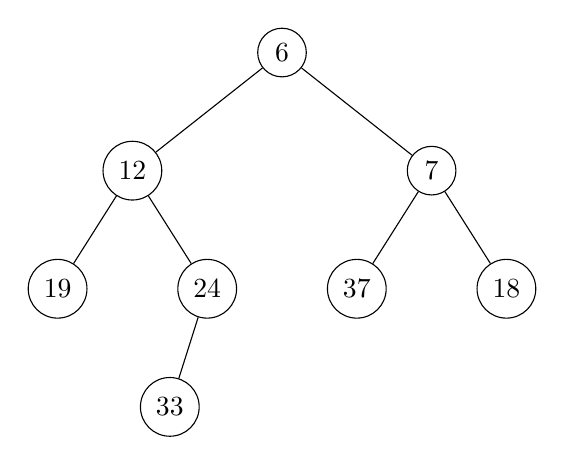
\begin{tikzpicture}[level distance=1.5cm,
			level 1/.style={sibling distance=3.8cm},
			level 2/.style={sibling distance=1.9cm},
			level 3/.style={sibling distance=0.95cm},
			every node/.style = {shape=circle, draw, align=center}]
			
			\node{6}
			child {node {12}
				child {node {19}}
				child {node {24}
					child {node {33}}
					child [missing]{}
				}
			}
			child {node {7}
				child {node {37}}
				child {node {18}}
			};
			\end{tikzpicture}
		\end{figure}
		\noindent Steg 1: nå ser vi at $ 6 < 8 $, dermed fletter vi venstre heap med høyre subheap av høyre heap:
		\begin{figure}[H]
			\centering
			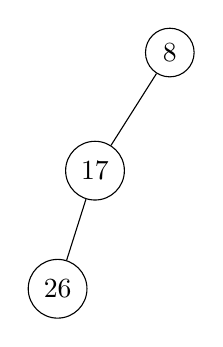
\begin{tikzpicture}[level distance=1.5cm,
			%level 1/.style={sibling distance=3.8cm},
			level 1/.style={sibling distance=1.9cm},
			level 2/.style={sibling distance=0.95cm},
			every node/.style = {shape=circle, draw, align=center}]
			
			
			\node{8}
			child {node {17}
				child {node {26}}
				child [missing] {}
			}
			child [missing]{};
			\end{tikzpicture}
			\quad\quad
			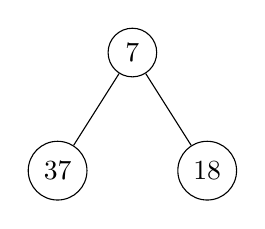
\begin{tikzpicture}[level distance=1.5cm,
			%level 1/.style={sibling distance=3.8cm},
			level 1/.style={sibling distance=1.9cm},
			level 2/.style={sibling distance=0.95cm},
			every node/.style = {shape=circle, draw, align=center}]
			
			\node{7}
				child {node {37}}
				child {node {18}};
			\end{tikzpicture}
		\end{figure}
		\noindent Steg 2: siden $ 7 < 8 $ fletter vi heapen til venstre med høyre subheap av heapen til høyre:
		\begin{figure}[H]
			\centering
			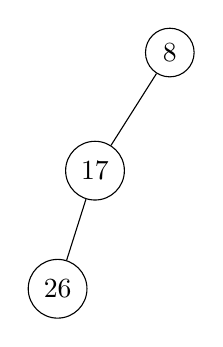
\begin{tikzpicture}[level distance=1.5cm,
			%level 1/.style={sibling distance=3.8cm},
			level 1/.style={sibling distance=1.9cm},
			level 2/.style={sibling distance=0.95cm},
			every node/.style = {shape=circle, draw, align=center}]
			
			
			\node{8}
			child {node {17}
				child {node {26}}
				child [missing] {}
			}
			child [missing]{};
			\end{tikzpicture}
			\quad\quad
			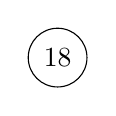
\begin{tikzpicture}[level distance=1.5cm,
			%level 1/.style={sibling distance=3.8cm},
			level 1/.style={sibling distance=1.9cm},
			level 2/.style={sibling distance=0.95cm},
			every node/.style = {shape=circle, draw, align=center}]
			
			\node{18};
			\end{tikzpicture}
		\end{figure}
		\noindent Steg 3: dette er trivielt, og blir basisen i rekursjonen. Vi fletter sammen heapene på vanlig måte:
		\begin{figure}[H]
			\centering
			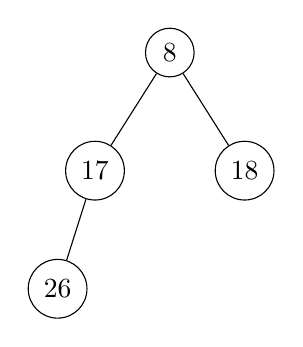
\begin{tikzpicture}[level distance=1.5cm,
			%level 1/.style={sibling distance=3.8cm},
			level 1/.style={sibling distance=1.9cm},
			level 2/.style={sibling distance=0.95cm},
			every node/.style = {shape=circle, draw, align=center}]
			
			
			\node{8}
			child {node {17}
				child {node {26}}
				child [missing] {}
			}
			child {node {18}};
			\end{tikzpicture}
		\end{figure}
		\noindent Nå begynner oppnøstingen i rekursjonen. Vi setter inn denne i steg 2 (erstatter høyre subheap i høyre heap med denne):
		\begin{figure}[H]
			\centering
			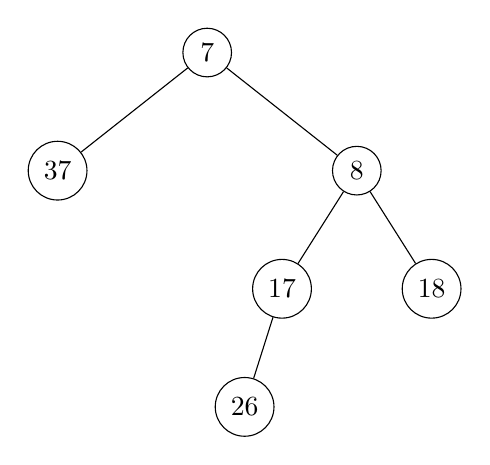
\begin{tikzpicture}[level distance=1.5cm,
			level 1/.style={sibling distance=3.8cm},
			level 2/.style={sibling distance=1.9cm},
			level 3/.style={sibling distance=0.95cm},
			every node/.style = {shape=circle, draw, align=center}]
			
			\node{7}
			child {node {37}}
			child {node {8}
				child {node {17}
					child {node {26}}
					child [missing] {}
				}
				child {node {18}}
			};
			\end{tikzpicture}
		\end{figure}
		\noindent Denne heapen oppfyller ikke krav 1 i definisjon \ref{def:leftheap}, vi må derfor swappe høyre og venstre supheap. Vi gjør dette og setter inn i steg 1:
		\begin{figure}[H]
			\centering
			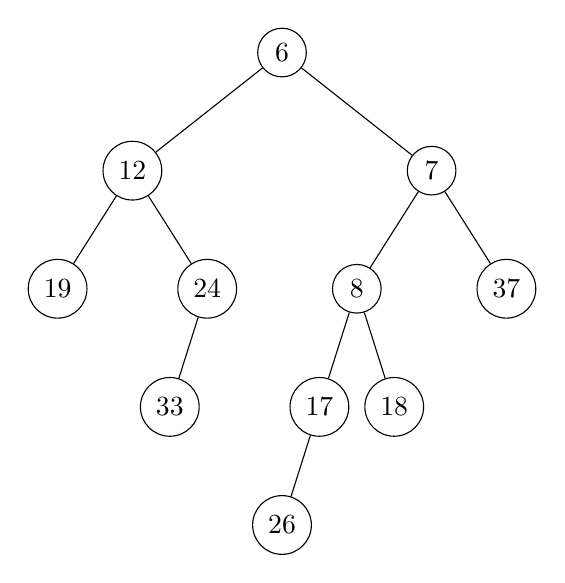
\begin{tikzpicture}[level distance=1.5cm,
			level 1/.style={sibling distance=3.8cm},
			level 2/.style={sibling distance=1.9cm},
			level 3/.style={sibling distance=0.95cm},
			every node/.style = {shape=circle, draw, align=center}]
			
			\node{6}
			child {node {12}
				child {node {19}}
				child {node {24}
					child {node {33}}
					child [missing]{}
				}
			}
			child {node {7}
			child {node {8}
				child {node {17}
					child {node {26}}
					child [missing] {}
				}
				child {node {18}}
			}
			child {node {37}}};
			\end{tikzpicture}
		\end{figure}
		\noindent Npl er 2 i begge subheaps, vi kan derfor sette rett inn i steg 0:
		\begin{figure}[H]
			\centering
			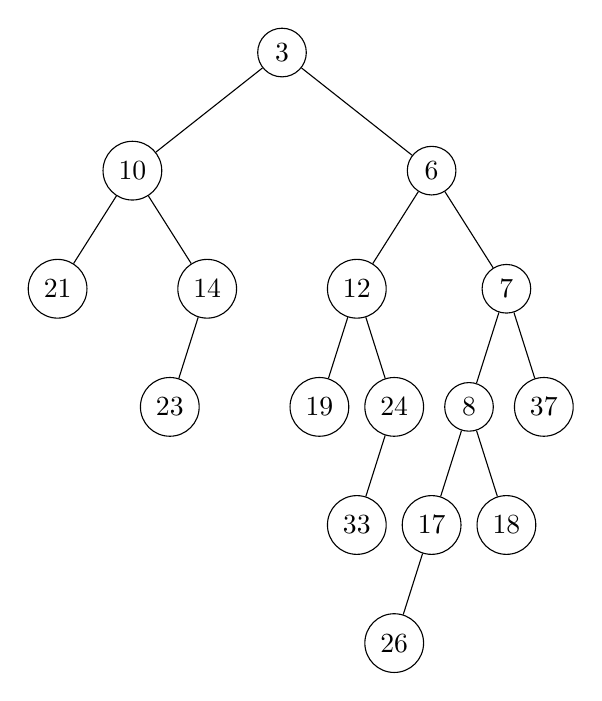
\begin{tikzpicture}[level distance=1.5cm,
			level 1/.style={sibling distance=3.8cm},
			level 2/.style={sibling distance=1.9cm},
			level 3/.style={sibling distance=0.95cm},
			every node/.style = {shape=circle, draw, align=center}]
			
			\node{3}
			child {node {10}
				child {node {21}}
				child {node {14}
					child {node {23}}
					child [missing]{}
				}
			}
			child {node{6}
			child {node {12}
				child {node {19}}
				child {node {24}
					child {node {33}}
					child [missing]{}
				}
			}
			child {node {7}
				child {node {8}
					child {node {17}
						child {node {26}}
						child [missing] {}
					}
					child {node {18}}
				}
			child {node {37}}}};
			\end{tikzpicture}
		\end{figure}
		\noindent Nå er vi nesten ferdige, vi ser at npl til venstre subheap er 1, og npl til høyre subheap er 2, vi må derfor swape venstre og høyre subheap:
		\begin{figure}[H]
			\centering
			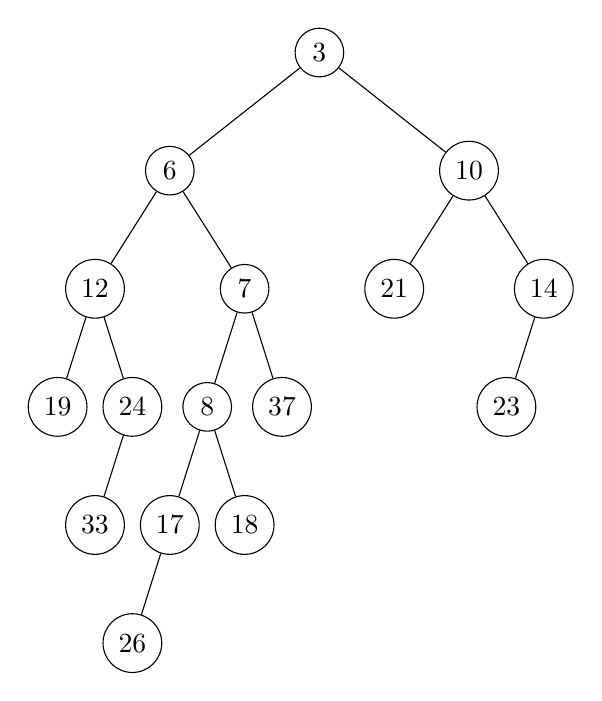
\begin{tikzpicture}[level distance=1.5cm,
			level 1/.style={sibling distance=3.8cm},
			level 2/.style={sibling distance=1.9cm},
			level 3/.style={sibling distance=0.95cm},
			every node/.style = {shape=circle, draw, align=center}]
			
			\node{3}
			child {node{6}
				child {node {12}
					child {node {19}}
					child {node {24}
						child {node {33}}
						child [missing]{}
					}
				}
				child {node {7}
					child {node {8}
						child {node {17}
							child {node {26}}
							child [missing] {}
						}
						child {node {18}}
					}
				child {node {37}}}}
			child {node {10}
				child {node {21}}
				child {node {14}
					child {node {23}}
					child [missing]{}
				}
			};
			\end{tikzpicture}
		\end{figure}
\end{example}
